

\newcommand{\summnu}{\Sigma m_\nu}
\newcommand{\FoM}{{\rm FoM}}
\newcommand{\cm}{\ \text{cm}}
\newcommand{\pc}{\ \text{pc}}
\newcommand{\Mpc}{\ \text{Mpc}}
\newcommand{\hMpc}{\ h^{-1}\text{Mpc}}
\newcommand{\hMpcc}{\ h^{-3}\text{Mpc}^3}
\newcommand{\ihMpc}{\ h\text{Mpc}^{-1}}
\newcommand{\iMpc}{\ {\rm Mpc}^{-1}}
\newcommand{\Ms}{\ M_\odot}
\newcommand{\hMs}{\ h^{-1} M_\odot}
\newcommand{\eh}[1]{\exp{\left[#1\right]}}
\newcommand{\tim}[1]{\times 10^{#1}}%times 10 
\newcommand{\unit}[1]{\ \text{#1}}
\newcommand{\tb}[1]{\textcolor{blue}{#1}}
\newcommand{\tr}[1]{\textcolor{red}{#1}}
\newcommand{\tsc}[1]{#1}
\newcommand{\derd}{\,\mathrm{d}} % upright d for derivatives and integrals
\newcommand{\ddir}{\delta^\text{(D)}}
\newcommand{\dkron}{\delta^\text{(K)}}
\newcommand{\be}{\begin{equation}}
\newcommand{\ee}{\end{equation}}
\newcommand{\la}{\left\langle}
\newcommand{\ra}{\right\rangle}
\newcommand{\derivd}{\text{d}}
\renewcommand{\vec}{\bm}
\newcommand{\dqc}{\frac{\derivd^3q}{(2\pi)^3}}
\newcommand{\dkpc}{\frac{\derivd^3k'}{(2\pi)^3}}
\newcommand{\dqcp}{\frac{\derivd^3q'}{(2\pi)^3}}
\newcommand{\dqcpp}{\frac{\derivd^3q''}{(2\pi)^3}}
\newcommand{\cyc}{\, \text{cyc.}}
\newcommand{\Dz}{\Delta z}
\newcommand{\Dv}{\Delta v}
\newcommand{\Dx}{\Delta x}
\newcommand{\Dtheta}{\Delta \theta}
\newcommand{\bz}{\bar{z}}
\newcommand{\kms}{{\rm km~s^{-1}}}

%bias parameters
\newcommand{\bdelta}{b_\delta}
\newcommand{\bdtwo}{b_{\delta^2}}
\newcommand{\bstwo}{b_{s^2}}
%renormalized fields
\newcommand{\msdtwo}{\left[\delta^2\right]}
\newcommand{\msstwo}{\left[s^2\right]}
%bold faced vectors
\newcommand{\vtheta}{\mathbf{\theta}}
\newcommand{\vv}{\mathbf{v}}
\newcommand{\vnabla}{\mathbf{\nabla}}
\newcommand{\vk}{\mathbf{k}}
\newcommand{\vr}{\mathbf{r}}
\newcommand{\vx}{\mathbf{x}}
\newcommand{\br}{\mathbf{r}}
\newcommand{\Tr}{\mathrm{Tr}}
\newcommand{\vxperp}{\mathbf{x_\perp}}
\newcommand{\vkperp}{\mathbf{k_\perp}}
\newcommand{\vrperp}{\mathbf{r_\perp}}
\newcommand{\vR}{\mathbf{r}}

%LyaF
%removed \ after several here - makes space before period - 
%add by hand when needed
\newcommand{\lya}{Ly$\alpha$}
\newcommand{\lyb}{Ly$\beta$}
\newcommand{\lyaf}{Ly$\alpha$ forest}
\newcommand{\vdf}{{\mathbf \delta_f}}
\newcommand{\lr}{\lambda_{{\rm rest}}}
\newcommand{\PF}{$P_F^{\rm 1D}(k_\parallel,z)$}
\newcommand{\bF}{\bar{F}}

%journals
\newcommand{\mnras}{{\em Mon. Not. Roy. Astron. Soc. }}
\newcommand{\apjl}{{\em Astrophys. J. Let. }}
\newcommand{\apj}{{\em Astrophys. J. }}
\newcommand{\apjs}{{\em Astrophys. J. Sup. }}
\newcommand{\jcap}{{\em JCAP }}
\newcommand{\physrep}{{\em Phys. Rept. }}
\newcommand{\aap}{{\em Astron. Astrophys. }}
\newcommand{\aj}{AJ }
\newcommand{\pasp}{PASP}
\newcommand{\prd}{PRD}
\def\pr{{Phys.\ Rev.\ }}
\def\astropart{{Astro-particle Phys.~}}
\def\rvmp{{Rev.\ Mod.\ Phys.\ }}

\def\pvm#1{[PM: {\it #1}] }
\def\af#1{[AF: {\it #1}] }


Forseeable  cosmological measurements can determine the sum of the 
neutrino masses, but not directly the separate contributions of the three species. However, if the hierarchy is normal with the sum of 
masses near the minimum of about 0.06 eV,
strong evidence for this should accumulate through the next decade, 
as expected large-scale structure/gravitational lensing experiments 
(Euclid, LSST, MS-DESI/BigBOSS, etc) come online. However, should the sum turn out to be about 0.10 eV or more, no conclusion could be drawn about the hierarchy.
Fortunately, the constraints on the neutrino masses are a byproduct of
experiments primarily motivated by dark energy studies, so they
will happen independent of neutrino-science considerations.

Neutrinos decouple from other particles very early and become
non-relativistic quite late, $z_{\rm nr}\sim 83~(m_\nu / 0.05~ {\rm
eV})$, relative to the time CMB was imprinted, $z=1100$.  The masses
of the neutrinos affect the fundamental cosmological observable, the
power spectrum.  The power spectrum is the Fourier transform of the
two-point correlation function between mass density at one point and
mass density at another point.  To be sure, we are talking about
cosmological separations.  The density of galaxies can stand as a
proxy for the density of matter, both ordinary and dark.   



Fig.~\ref{fig:powerratio} shows the
ratio of power for $\summnu=0.11$ eV to $\summnu=0.06$ eV as a function of 
$k$, the Fourier transform variable measured in ${\rm Mpc}^{-1}$.
\begin{figure}[bp]
\vspace{-0.6cm}
  \centering
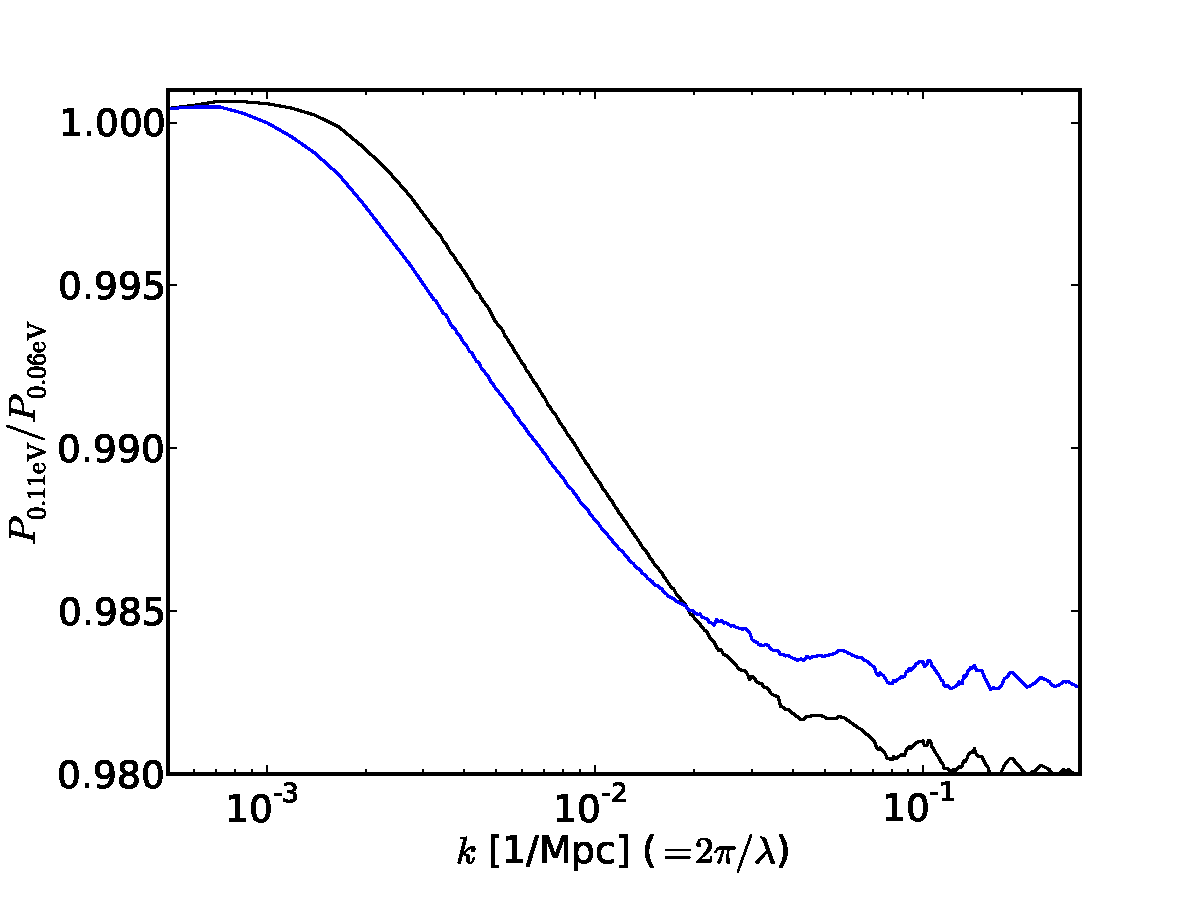
\includegraphics[width=0.6\textwidth]{PM/neutrinosCAMB.pdf}
\vspace{-0.2cm}
\caption{
Ratio of linear power for $\summnu=0.11 {\rm eV}$ in the inverted (black) or
normal (blue) hierarchy, to $\summnu=0.06{\rm eV}$ in the normal hierarchy.
}
\label{fig:powerratio}
\end{figure}
Fig.~\ref{fig:powerratio} illustrates the small differences in power spectra for different 
distributions of
the total mass between particles, but these are not expected to be observable
on the time scale under consideration~\cite{2006PhRvD..73l3501S}.
The dominant effect that can be measured is the suppression in power shown
in Fig.~\ref{fig:powerratio}. Note, however, that it is not necessary to rely 
entirely on measuring the effect on the {\it shape} of the power spectrum shown
in Fig.~\ref{fig:powerratio}. Redshift-space 
distortions, lensing, and other methods can be used to measure the overall 
suppression
in amplitude relative to the CMB measurement of the primordial perturbations 
(this relies, however, on GR calculations of the growth of structure).



There are numerous ways to detect the large-scale power suppression by 
neutrinos, with varying degrees of statistical power and expected 
systematic uncertainties. 
The focus here is on galaxy redshift surveys, which appear to offer the best 
combination of statistical power and projected control of systematic effects.

The first major redshift survey that may seriously test the hierarchy is 
MS-DESI (approximately equivalent to BigBOSS \cite{2011arXiv1106.1706S}). 
Led by LBNL, the survey will cover $\sim 14000$ square 
degrees, 
taking spectra of $\sim 20$ million galaxies and quasars at $z\sim 0-3$. 
MS-DESI is likely to run on the Mayall 4~m telescope at Kitt Peak National 
Observatory near Tucson, AZ, over a $\sim5$ year period from 
2018 to 2022. It is possible that the spectrograph could then be moved to the
twin Blanco telescope in Chile to cover another $\sim 10000$ square degrees.

Another big redshift survey that appears certain to happen is the 
European-led Euclid satellite \cite{2012SPIE.8442E..0ZA}. 
Euclid will measure redshifts for 
$\sim 50$ million galaxies over $\sim 15000$ square degrees.  
The target survey period is $\sim 2020-2026$. In addition to redshifts, 
Euclid will do imaging for gravitational lensing measurements.

While not a redshift survey (meaning it has limited radial resolution), LSST
will be a major US cosmological experiment running in the 2022-2032 time 
period \cite{2009arXiv0912.0201L}.
It will image $\sim 20000$ square degrees for gravitational lensing,
which can add  power 
to the redshift survey measurements of neutrino masses.
Before LSST, and even before MS-DESI, there will be a smaller, 5000 sq. deg.
lensing survey, DES
(\url{http://www.darkenergysurvey.org}). 
We add DES to all projections that do not include LSST. 

Another experiment that {\em might} happen is the NASA/WFIRST satellite, 
intended for a 2022 launch \cite{2012arXiv1208.4012G}. 
It would be qualitatively similar to MS-DESI and
Euclid, but complementary ($i.e.$ adding statistical power) because it would
take a different strategy of going deeper over a smaller area.    


Projections are given in Table~\ref{tablemnulensing}.
\begin{table}[b]
\caption{ 
Potential constraints on 
$\Sigma m_{\nu}$ for the minimal parameter set.
``P'' means Planck CMB data has been included.
Numbers in parentheses are maximum $k$ used for galaxy clustering, in units of
$\iMpc$. 
BigBOSS14 / 24 means 14000 or 24000 square degrees (BigBOSS is later shortened to BB). 
From the Euclid satellite (sometimes shortened to Euc) 
only the redshift space clustering information is used, not lensing.
The $\sigma_{0.04~{\rm eV}}$ column shows the detection significance for a
mass difference of $0.04$ eV, corresponding to the hierarchy detection 
significance {\em if} the total mass is absolutely minimal.
DES and LSST stand for the lensing and galaxy clustering components of these 
surveys. 
\label{tablemnulensing}}
\vspace{-0.3cm}
\begin{center}
\begin{tabular}{lcccc}
\hline
$ $ & $k_{\rm max}$ & $\sigma_{\Sigma m_{\nu}}$ & $\sigma_{0.04~{\rm eV}}$ & 
Year \\
$ $ & $\left[\iMpc\right]$ & $\left[{\rm eV}\right]$ & &  \\
\hline
P+BigBOSS14+DES & 0.07 & $0.021$ & 1.9 & 2022 \\
P+Euclid+DES & 0.07 & 0.019 & 2.1 & 2026 \\
P+BigBOSS24+DES & 0.07 & $0.019$ & 2.1 & 2026 \\
P+BB24+Euc+DES & 0.07 & $0.016$ & 2.5 & 2026 \\
P+BB24+Euc+LSST & 0.07 & $0.014$ & 2.9 & $\lesssim 2030$  \\
P+BB14+DES & 0.14 & $0.017$ & 2.4 & 2022 \\
P+Euclid+DES & 0.14 & $0.015$ & 2.9 & 2026 \\
P+BB24+DES & 0.14 & $0.015$ & 2.7 & 2026 \\
P+BB24+Euc+DES & 0.14 & $0.013$ & 3.1 & 2026 \\
P+BB24+Euc+LSST & 0.14 & $0.011$ & 3.6 & $\lesssim 2030$ \\
\hline
\end{tabular}
\end{center}
\vspace{-0.3cm}
\end{table}
As shown, cosmology can generally achieve or at least approach the 
$0.01$ eV RMS error level needed to probe the hierarchy. 
These calculations are consistent with similar projections made for
Euclid~\cite{2013JCAP...01..026A}. 


As seen in Table~\ref{tablemnulensing}, cosmology is 
likely to reach the $2-2.5~\sigma$ level for distinguishing the minimal normal 
from minimal inverted hierarchies by the end of MS-DESI (in the North at 
least) in 2022. At that point
Euclid and LSST will be running, and significance will accumulate, probably 
reaching the $\sim 3.5~\sigma$ level around 2026 (LSST will only be half-done 
at that
point, but most of the gain from it will likely be extractable already).
Whether these measurements will determine the neutrino mass hierarchy is contingent on the hierarchy being normal and the masses minimal.  
